\section{Kasus Numerik pada Lingkungan Qiskit}

\begin{frame}{Implementasi \textit{Quantum Phase Estimation} (QPhE)}
    \begin{columns}
        \begin{column}{0.5\textwidth}
            \begin{itemize}
                \item Algoritma iteratif \textit{Quantum Phase Estimation} menyandikan nilai probabilitas fase \textit{eigenvalue} mengandalkan register 3-bit komputasi secara simultan.
                \item \textit{Initial state} dideterminasi presisi menggunakan amplitudo fasa non-trivial untuk mengawali \textit{profiling} volatilitas ekuivalen data riwayat finansial.
                \item Gambar di samping mengilustrasikan evolusi sirkuit QPhE yang diposisikan di bawah dominasi gerbang \textit{Controlled-Unitary} ($CU$) dengan variabel rotasi internal $(\theta, \phi, \lambda)$ spesifik yang menyebabkan fenomena \textit{phase kickback}.
            \end{itemize}
        \end{column}
        \begin{column}{0.5\textwidth}
            \begin{figure}
                \centering
                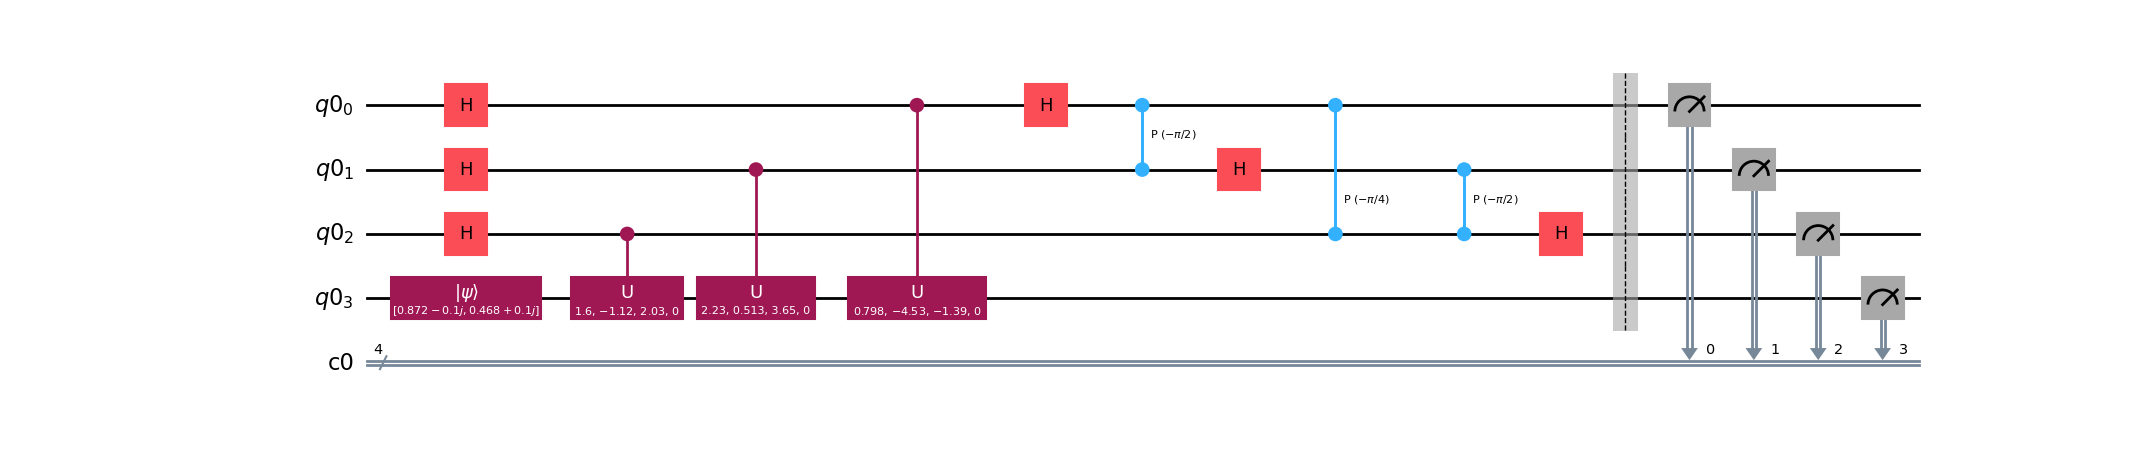
\includegraphics[width=\textwidth,keepaspectratio]{QPCA-master/circuit_qphe.png}
                \caption{Topologi sirkuit kuantum untuk eksekusi QPhE.}
            \end{figure}
        \end{column}
    \end{columns}
\end{frame}

\begin{frame}{Proses Transpilasi Gerbang Sirkuit (\textit{Transpilation})}
    \begin{figure}
        \centering
        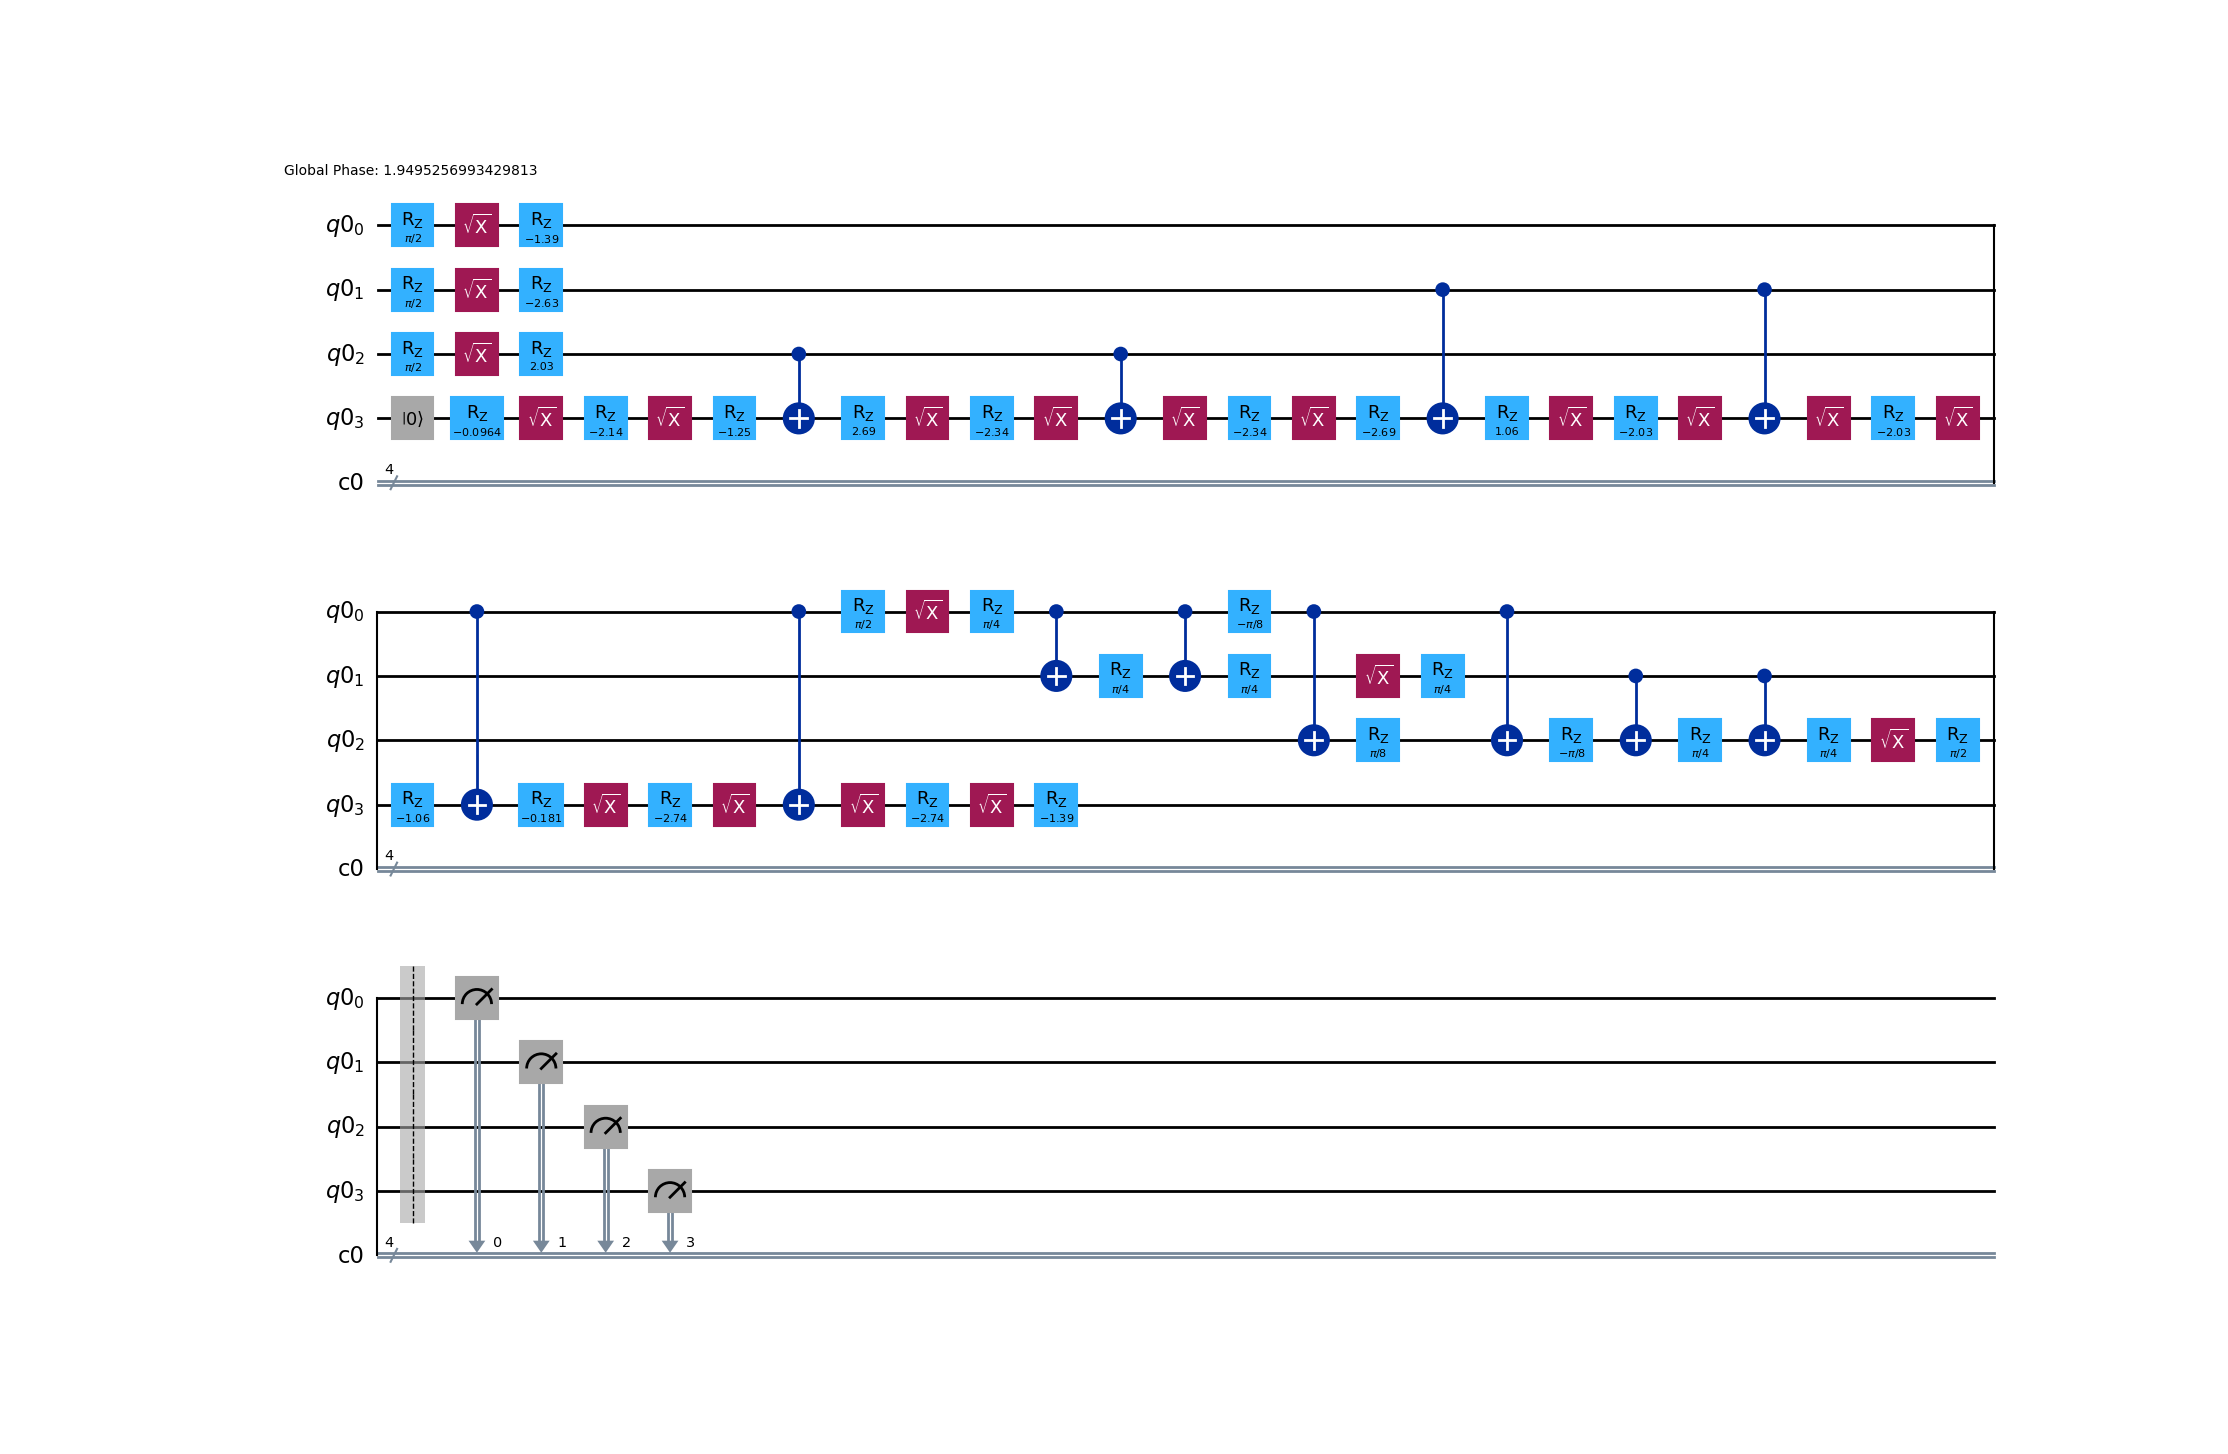
\includegraphics[width=0.8\textwidth,keepaspectratio]{QPCA-master/circuit_transpiled_qphe.png}
        \caption{Transpilasi elemen gerbang uniter tingkat tinggi menuju gerbang basis \textit{hardware}.}
    \end{figure}
    \begin{itemize}
        \item Gambar di atas mengilustrasikan reduksi kompilasi program menjadi interaksi dasar antar-qubit (\textit{inter-qubit routing}) yang eksklusif menggunakan representasi $U3$ dan sekuens interaksi matriks CNOT ($CX$).
        \item Pemetaan mikroskopis ini menelanjangi kedalaman sirkuit absolut (\textit{circuit depth}), mendemonstrasikan efisiensi algoritma sejati sebelum diproses langsung oleh \textit{noisy physical hardware}.
    \end{itemize}
\end{frame}

\begin{frame}{Verifikasi Sirkuit Menggunakan \textit{Eigenstate} Murni}
    \begin{columns}
        \begin{column}{0.5\textwidth}
            \begin{itemize}
                \item Gambar di samping mengilustrasikan sirkuit validasi alternatif dengan resolusi fase lebih rendah (2-bit) dipasangkan secara artifisial dengan matriks \textit{pure target state} $|+\rangle$.
                \item Deskalasi \textit{overhead} komputasi membatasi penyebaran galat sistematis (\textit{gate error propagation}), memastikan pergerakan interferensi algoritmik fasa murni dapat tercapai dengan tajam secara optikal maupun probabilitas.
            \end{itemize}
        \end{column}
        \begin{column}{0.5\textwidth}
            \begin{figure}
                \centering
                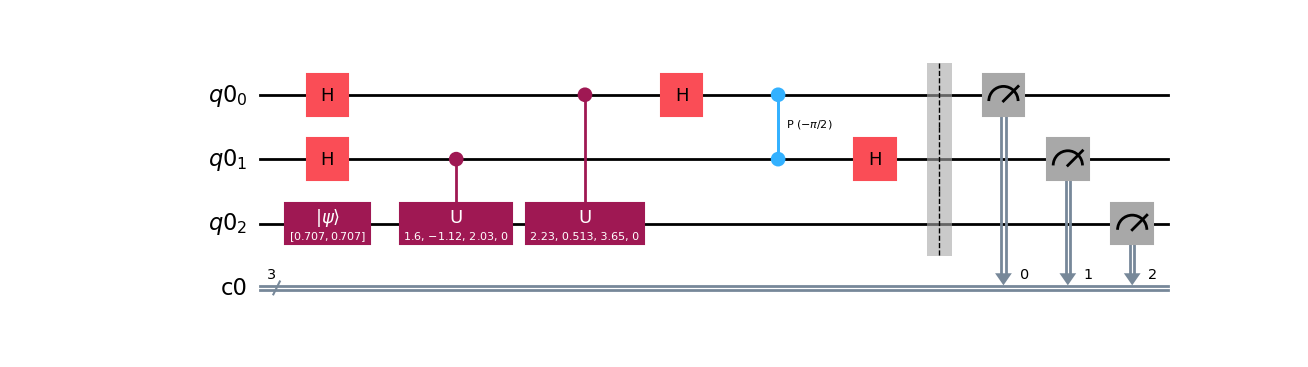
\includegraphics[width=\textwidth,keepaspectratio]{QPCA-master/circuit_eigenstate.png}
                \caption{Arsitektur validasi gerbang menggunakan input superposisi seragam.}
            \end{figure}
        \end{column}
    \end{columns}
\end{frame}

\begin{frame}{Skalabilitas Beban Komputasi Matriks Kovarians $4 \times 4$}
    \begin{figure}
        \centering
        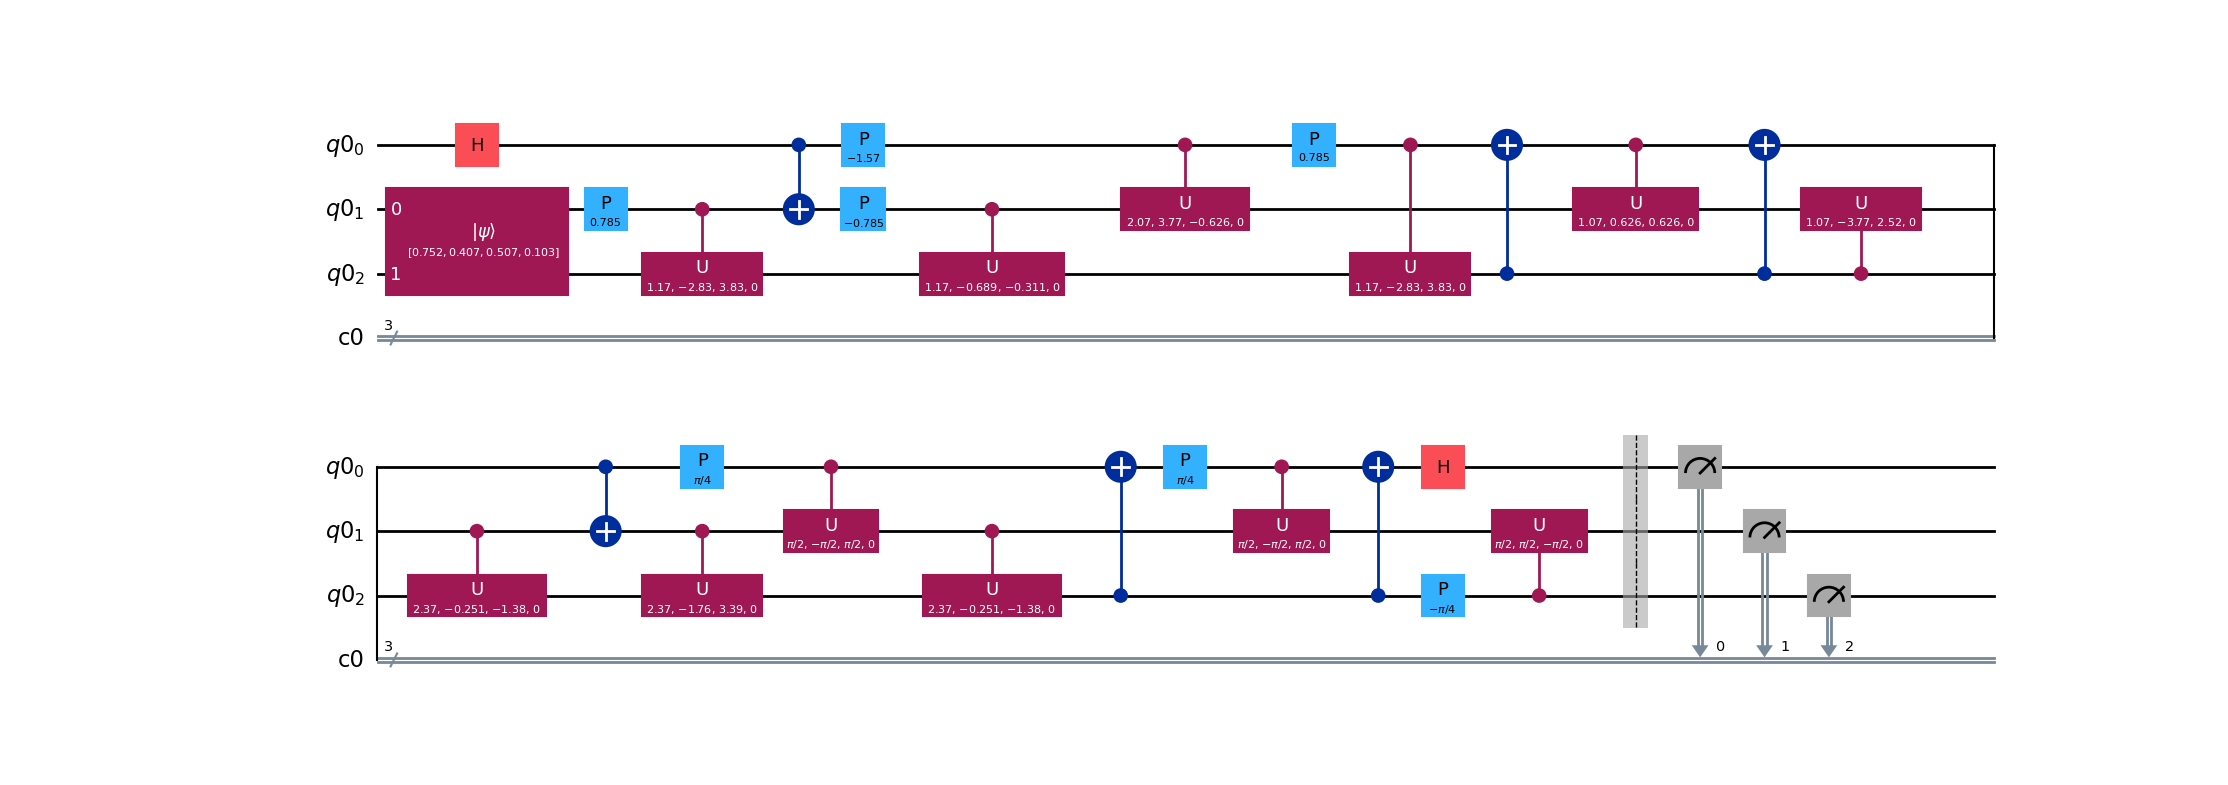
\includegraphics[width=0.7\textwidth,keepaspectratio]{QPCA-master/circuit_4x4.png}
        \caption{Ekspansi desain arsitektural qPCA untuk instrumen sistem $4 \times 4$.}
    \end{figure}
    \begin{itemize}
        \item Gambar di atas mengilustrasikan eskalasi kompleksitas pada dinamika matriks korelasi $\rho_4$, di mana struktur mensyaratkan 28 urutan gerbang uniter (meliputi 12 matriks interaksi \textit{Controlled-Unitary}).
        \item Ekspansi drastis pada \textit{circuit depth} memunculkan tantangan fundamental terhadap \textit{baseline} resistansi koherensi yang dimiliki spesifikasi qubit era NISQ.
    \end{itemize}
\end{frame}
